%\setcounter{chapter}{35}
\chapter{Computer Vision and Society}
\label{chapter:computer_vision_and_society}


\section{Introduction}

The success of computer vision has led to vision algorithms playing an
ever-larger role in society. Face recognition algorithms unlock
our phones and find our friends and family members in photographs;  cameras identify
swimmers in trouble in swimming pools and assist people in driving
cars.

With such a large role in society, one may expect that computer vision mistakes can
have a large impact and have the potential to cause harm, and
unfortunately this is true.  While self-driving cars may save tens of
thousands of lives each year, mistakes in those algorithms can also
lead to human deaths.  A mistaken computer match with a surveillance
photograph may implicate the wrong person in a crime.  Furthermore,
the performance of computer vision algorithms can vary from person to
person, sometimes as a function of protected attributes of the person, such as gender, race, or age.
These are potential outcomes that
the computer vision community needs to be aware of and to
mitigate.

The field of {\bf Algorithmic Fairness}\index{Algorithmic Fairness} studies the performance and fairness
of algorithms across people, groups, and cultures.  It seeks to
address algorithmic biases, and to develop strategies to ensure that computer vision algorithms don't reflect or create biases against different groups of people or cultures.
Entry points to this literature include a number of text and video sources, including \cite{Kearns2020,Gebru2020,Hamidi2018,Garvie2016,Hutchinson2019,Dwork2012,barocas-hardt-narayanan,Hardt2020}.

We review two topics: fairness and ethics.
In \sect{\ref{sect:fairness}}, we describe some current techniques.  This is just a small sampling of work in this quickly evolving area, selected to intersect well with the material in the rest of this book.  There is more literature and more subtleties than can be covered here. Even if our algorithms and datasets were completely free of bias, there are still many ethical concerns regarding the use of computer vision technology.
In \sect{\ref{sect:ethics}}, we pose ethics questions that we encourage computer vision researchers to think about.


\section{Fairness}
\label{sect:fairness}

Modern computer vision algorithms are trained from data, and thus are
influenced by the statistical make-up of the training data.
Correlations between the expressed gender of
individuals and their depicted activities recorded within a dataset
can perpetuate or even amplify societal gender biases captured in the dataset \cite{Zhao2017,dalessandro2017,Noble2018}.  Gender classification systems in 2018 showed performance that depended on skin tone \cite{Buolamwini2018}.


There is a need for datasets, and the algorithms trained from them, to minimize spurious relations between protected attributes of people, such as skin color, age, gender, and the image labels or recognition outputs, such as occupation or other qualities that should not depend on the protected attributes.
Researchers have begun to develop methods to identify and mitigate such biases in either computer vision databases or algorithms.

\subsection{Facial Analysis}

Facial detection asks whether there is a face in some image region, while facial analysis refers to measuring additional attributes of the face, including pose and identity.  It is important to characterize the performance of facial analysis systems across demographic groups, as certain studies have done \cite{Klare2012}.  A large Face Recognition Vendor Test by the National Institute of Standards and Technology (NIST) \cite{Grother2019}  examined the accuracy of face recognition algorithms for different demographic groups defined by sex, age, and race or country of birth. For one dataset, they found
false positive rates were highest in West and East African and East Asian people, and lowest in Eastern European individuals. For the systems offered by many vendors, this effect was large, with differences of up to a factor of 100 in the recognition false positive rates between different countries of birth. In addition, the more accurate face recognition systems showed less bias and
some developers supplied highly accurate identification algorithms for
which false positive differentials were undetectable.
Certain studies \cite{Grother2019} have stressed the importance of reporting both false negative and false positive rates for each
demographic group at that threshold. Others \cite{Cavazos2021} have provided
a checklist for measuring bias in face recognition algorithms.  It is clearly important to understand the biases of any facial analysis system that is put into use, as these characteristics can vary greatly from system to system.

%% https://arxiv.org/pdf/1904.07325.pdf
%% Characterizing the Variability in Face Recognition Accuracy Relative to Race


\subsection{Dataset Biases}
\index{Dataset bias}

One cause of algorithmic bias can be a bias in the contents of the training dataset.
There are many subtleties in the creation and labeling of computer vision datasets \cite{Ramaswamy2021b}.
Any dataset represents only one slice of the possible images and labels that one could capture from the world \cite{Torralba2011}.
Furthermore, the samples taken may well be influenced by the background of the researchers gathering the dataset.
\Fig{\ref{fig:soap}} shows examples of common objects from four different households across the globe.  From left to right, the photographs are shown in decreasing order of the average household income of the region from which the photo was taken.  The object recognition results for six different commercially available image recognition systems are listed below each photograph, showing that the performance is much better for the images from first-world households \cite{DeVries2019},  possibly due to a better representation of imagery from such households in the training datasets of the image recognition systems.

\begin{figure}[t]
  \centerline{
    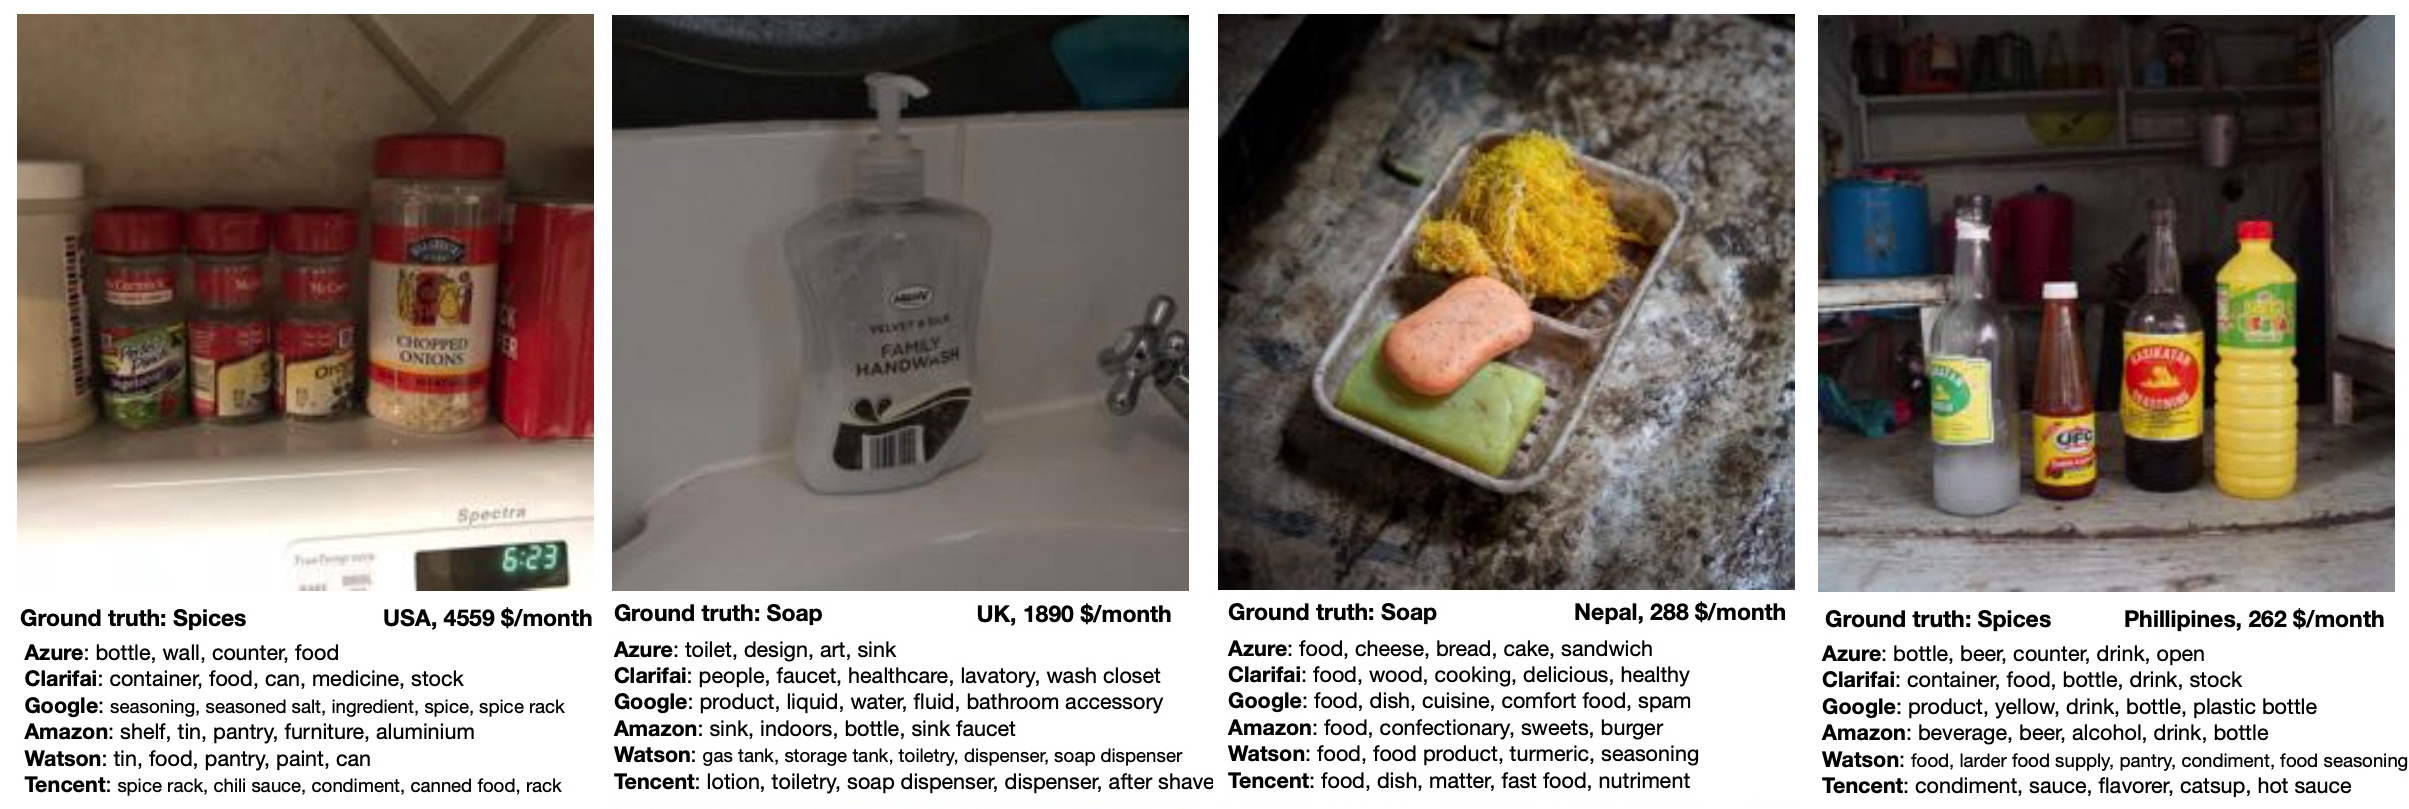
\epsfig{file=figures/fairness/soap3.jpg,width=1\linewidth}}
  \caption{Images of household items, and their recognized classes by five object recognition systems \cite{DeVries2019}. The systems tend to perform worse for non-Western countries and for lower-income households, such as those of the right two photographs.}
  \label{fig:soap}
\end{figure}



\subsection{Generative Adversarial Networks to Create Unbiased Datasets and Algorithms}

One way to mitigate a biased dataset is to synthetically produce the images needed to provide the necessary balance or coverage.
Generative adversarial networks (GANs), described in \chap{\ref{chapter:generative_models}}, can operate on a dataset  to generate sets of images similar to those of the dataset, but differing from each other in controlled ways, for example, with changes in the apparent gender, age, or race of depicted people.  Such GANs  have been used to develop debiased datasets and algorithms.

Sattigeri et al. \cite{Sattigeri2019} proposed an algorithm they called Fairness GAN, which included a classifier trained to perform {\em as poorly as possible} on predicting the classification result based on a protected attribute.  For example, the algorithm was designed to predict an attractiveness label while gaining no benefit from knowing the gender or skin tone.  The resulting debiased dataset showed some improvement in fairness metrics.

Another study \cite{Ramaswamy2021}  took an alternative approach to the problem of removing correlations between a protected attribute and a target label.  The authors  used GANs to generate pairs of realistic looking images that were balanced with respect to each protected attribute.  \Fig{\ref{fig:augmentation}} shows an example of this.  If ``wearing hat'' is deemed to be the protected attribute, it is desired to remove its correlation in the data with the attribute, ``wearing glasses.'' If no debiasing steps were taken, the algorithm would learn to associate wearing hats with wearing glasses.  The GAN is used to augment the dataset with paired examples of images of people wearing hats both with and without glasses.
When this augmented dataset is combined with the original dataset, performance in a variety of fairness measures is improved.

Still another approach to dataset fairness, by \cite{Zhao2017},
injects constraints to require that the model predictions follow the
distributions observed within the
training data, assuming that the training data has the desired distribution.
See also \cite{Wang2020} for a  benchmark and comparison of techniques for dataset bias mitigation.

\begin{figure}[t]
  \centerline{
    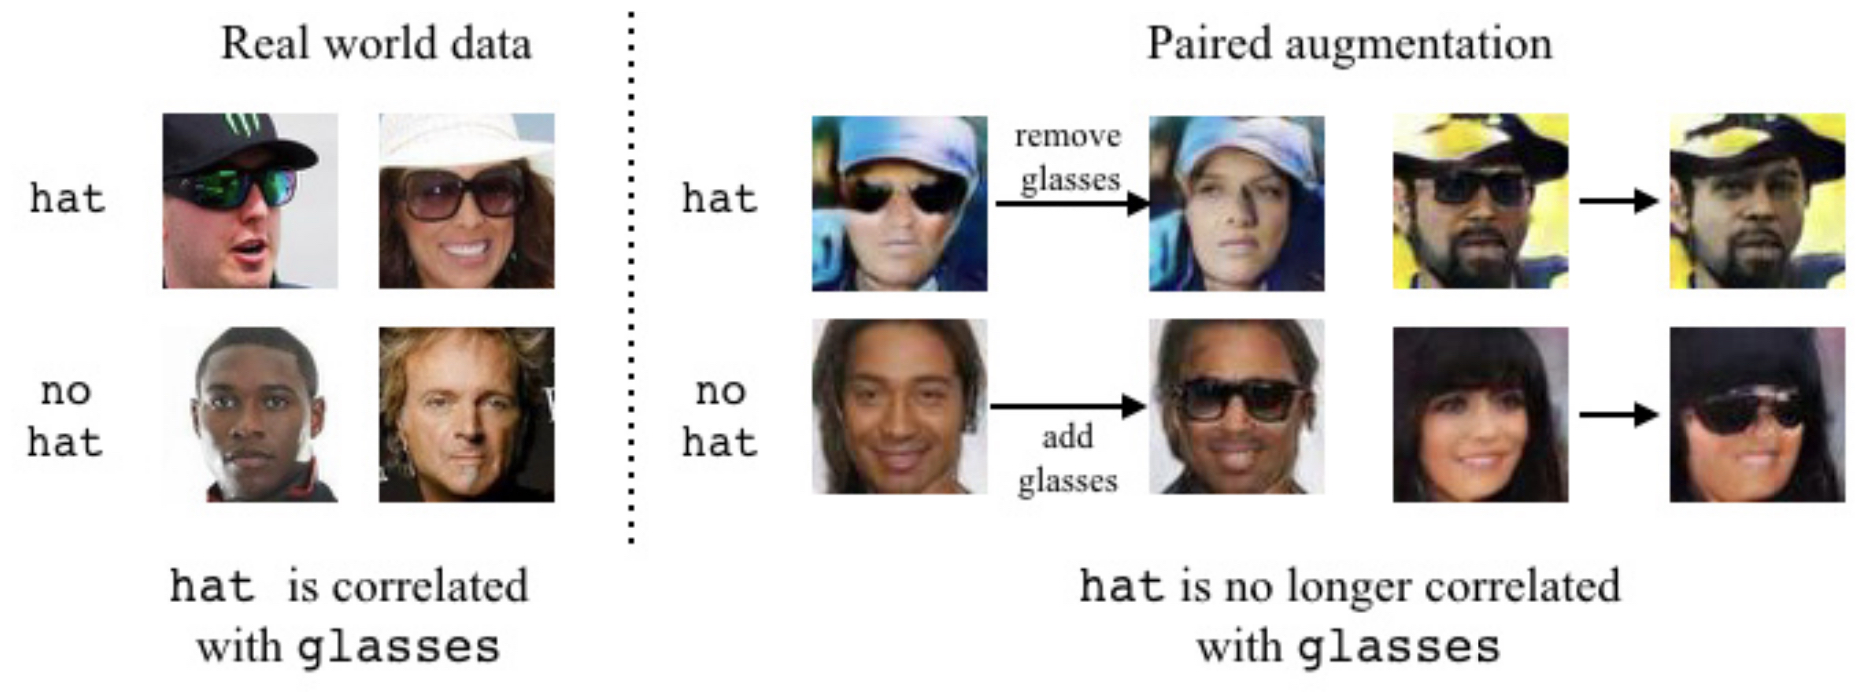
\epsfig{file=figures/fairness/augmentation.jpg,width=1\linewidth}}
  \caption{In this example ``wears hat'' is deemed to be a protected attribute, but it is correlated with another attribute, which in this example is ``wears glasses'' \cite{Ramaswamy2021}. The GAN-based method generates sets of images where wearing hats is not correlated with wearing glasses.}
  \label{fig:augmentation}
\end{figure}


\subsection{Counterfactuals for Analyzing Algorithmic Biases}

It may be difficult to distinguish whether a given biased result is caused by algorithmic bias or by biases in the testing dataset \cite{Balakrishnan2020}.  One way to disentangle those is through experimentation, that is, modifying variables of a probe image and examining the algorithm's decision.  GAN models, when coupled with human labeling to learn directions in the latent space corresponding to changes in the desired attributes, allow for such experimental intervention. Researchers \cite{Balakrishnan2020} have shown that such counterfactual studies may lead to very different conclusions than observational studies alone, which can be influenced by biased correlations in the testing dataset.  (See also related work in counterfactual reasoning by \cite{Denton2019}.)  \Fig{\ref{fig:transect}} shows several {\bf transects} from \cite{Balakrishnan2020}, paths through the GAN's latent space where only one face variable is modified. The variation in an algorithm's classification results along the images of the transect to provide a clean assessment of any bias related to the variable being modified.

\begin{figure}[h!]
  \centerline{
    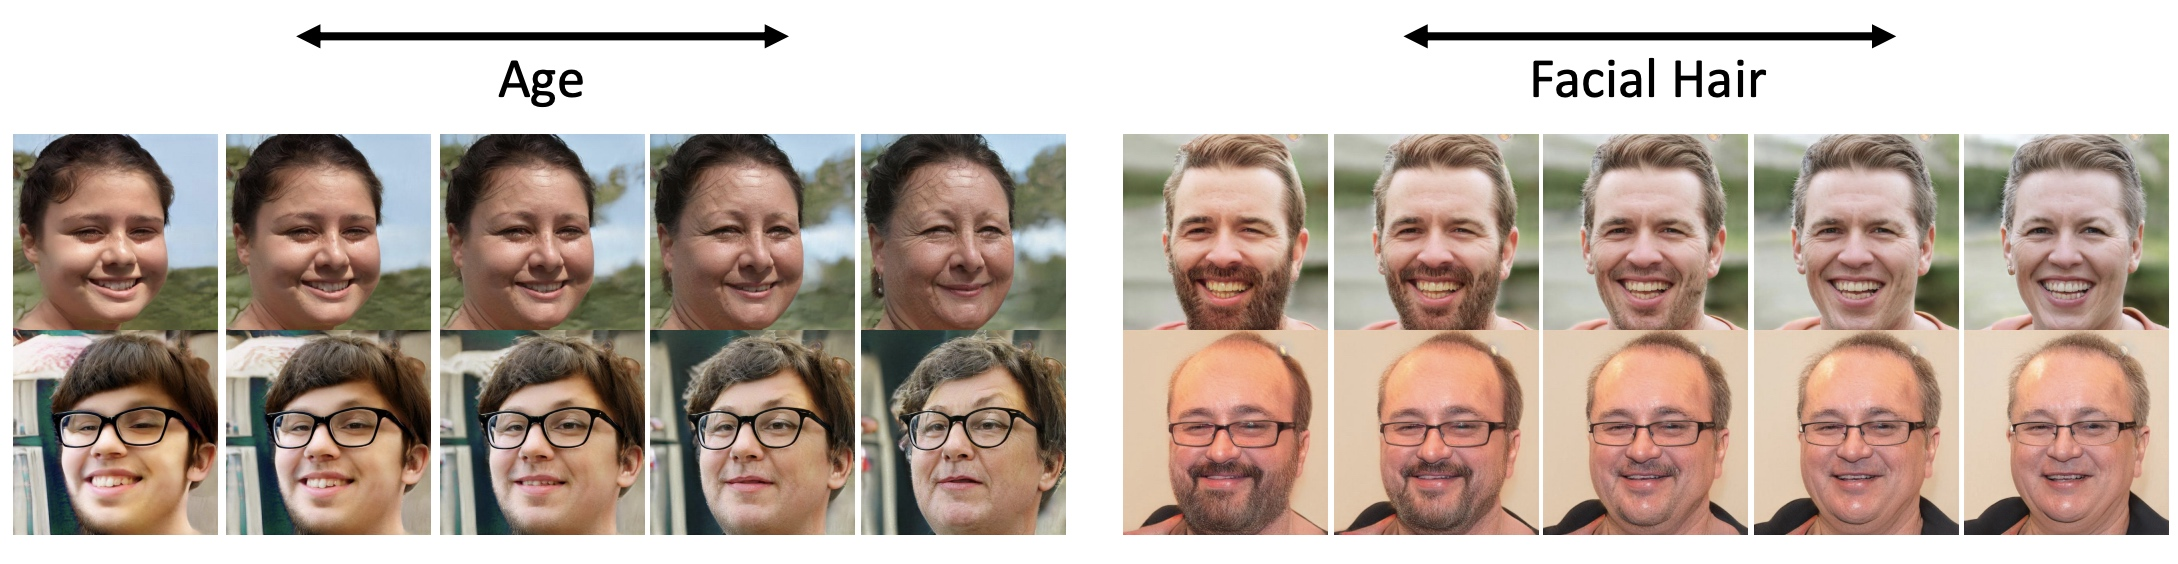
\epsfig{file=figures/fairness/transect.jpg,width=1\linewidth}}
  \caption{
    %When combined with human labeling to learn directions in the latent space corresponding to desired variables, a GAN can generate {\bf transects}, sequences of face images where only one variable changes. 
    A GAN creates sequences of faces, called {\bf transects}, where only one attribute changes \cite{Balakrishnan2020}.
    %This is done by using human labeling to learn how to make changes in the desired parts of the images. These sequences are called "transects".
    %Resulting algorithmic performance then directly indicates biases.
  }
  \label{fig:transect}
\end{figure}



\subsection{Privacy and Differential Privacy}

Since progress in computer vision often comes via new datasets, which typically show images and activities of people, issues of privacy are very important in computer vision research.  There are many ways in which people can be harmed by either intentional or unintentional participation in a dataset.  Datasets of medical results, financial transactions, views of public places, all can contain information that must remain private.
Conversely, there is a benefit to society of releasing datasets for researchers to study:  associations can be found that will benefit public health or safety.  Consequently, subjects want researchers to work with anonymized versions of their datasets.  Unfortunately, a number of well-known examples have shown that seemingly cleaned data, when combined with another apparently innocuous dataset, can reveal information that was desired to be private.  For example, in 1997, the medical records of the governor of Massachussetts were identified by matching anonymized medical
data with publicly available voter registration records \cite{Kearns2020,Dwork2014}.
%% (but see \cite{Barth-Jones2012} for nuances to the story).  
The combination of the two datasets allowed seemingly de-identified private data to be re-identified.


A very successful theoretical privacy framework, called differential privacy, addresses these issues.
Following the techniques of differential privacy \cite{Dwork2014}  researchers can guarantee to the participants of a study that they will not be affected by allowing their data to be used in a study or analysis,
no matter what other studies, datasets, or information sources are available.

\marginnote{ {\bf Differential privacy} allows extracting aggregated information about a population from a database without revealing information about any single individual.}

Algorithms can be designed for which it can be shown that the guarantee of differential privacy is met
\cite{Kearns2020,Dwork2014}.  One approach is to inject enough randomness into each recorded observation to guarantee that no individual's data can be reconstructed (with probabilistic guarantees that can be made as stringent as desired, at the cost of data efficiency), while still allowing scientific conclusions to be formed by averaging over the many data samples.
A simple example of this approach, described in \cite{Kearns2020}, is the following procedure to query a set of adults to determine what fraction of them have cheated on their partner.  Each surveyed adult is instructed to flip a coin.  If the coin shows heads, they are instructed to answer the question, ``Have you cheated on your partner?'',  truthfully.  If the coin shows tails, they are asked to answer ``yes'' or ``no'' at random, by flipping the coin again and answering ``yes'' if heads and ``no'' if tails.  The resulting responses for each individual are stored.



If the stored data were hacked, or accidentally leaked, no harm would come to the surveyed individuals even though their data from this sensitive survey had been revealed.  Any ``yes" answer could very plausibly be explained as being a result of the subject having been instructed by the protocol to flip a coin to select the answer.  Yet it is still possible to infer the true percentage of ``yes" answers in the surveyed population from the stored data:  the expected value of the measured percentages will be the true ``yes" and ``no" answers in the population.  The price for this differential privacy is that more data must be collected to obtain the same accuracy guarantees in the estimate of the true population averages.

\marginnote{There are also risks associated with the wrong use of differential privacy \cite{Dwork_Kohli_Mulligan_2019}.}

\section{Ethics}
\label{sect:ethics}

Many ethical issues are outside of the traditional training and education of scientists or
engineers, but ethics are important for vision scientists to think
through and grapple with.  Scientists have a distinguished history of engaging
with ethical and moral issues
\cite{Huxley1932,Orwell1948,Kearns2020,Rogaway2015}.

\subsection{Concerns beyond Algorithmic Bias}

Suppose the research community developed algorithms that could recognize and analyze people or objects equally well, regardless of displayed gender, race, age, culture or other class attributes.  Is the community's work toward fairness completed?  Unfortunately, there are still many issues of concern, as pointed out by many authors and speakers \cite{Gebru2020,Gebru2021,Benjamin2019}.
To list a few of these issues:

\begin{itemize}
  \item Face analysis for job hiring.  Companies have used automated facial analysis methods (analyzing expressions and length of responses) as part of their proprietary algorithms for resume screening, although, at least for some cases, that process has stopped after criticism of the fairness of these methods for screening \cite{Kahn2021}.
  \item Automated identification of faces can be used to compile a list of the participants at a public protest, potentially allowing retribution for attendance
        \cite{Garvie2016,Mozur2019}.
  \item People can show a bias toward believing the output of a machine \cite{Cummings2004}, making it more difficult for a person to correct an algorithm's mistake.

  \item There are concerns whether labeling the gender of a person from their appearance could cause distress or harm to some in the LGBTQ community \cite{Hamidi2018,Bennett2021}.
\end{itemize}

We provide a subsequent list of
questions for thought and discussion.  We encourage computer vision students and
practitioners to engage with these questions, and, of course, to continue to ask their own questions as well.  We need to work both as technologists and as citizens to ensure that computer vision technologies are used responsibly.


\subsection{Some Ethical Issues in Computer Vision}

The following are an (incomplete) set of questions that researchers and engineers may keep in mind:

\begin{itemize}
  \item Would you prefer that a person identify someone from a
        photograph, with the potential biases and assumptions that the
        individual may have, or for an algorithm to do so, based on training
        from a dataset which may include biases of its own? See \cite{Kearns2020,Mullainathan2019} for related discussions.
  \item What privacy safeguards must be in place to accept always-on
        camera and voice recording inside people's homes?  Inside your own home?
  \item Traffic fatalities in the US currently result in the tragedy
        of approximately
        30,000 deaths annually, with most of those fatalities being caused by
        driver error. If every vehicle were self-driving, fatalities caused by human error could fall dramatically, yet there will surely still be fatalities caused by machine errors, albeit far fewer than had been caused by humans.  Is that a tradeoff society should make? What should be our threshold of fatalities caused by machine?
        This moral question is a societal-scale
        version of ``the trolley problem''\index{The trolley problem} \cite{Thomson1985}:  A bystander can choose to divert a trolley from the main track to a side track, saving five people who are on that main track, but killing one person who is on the side track.  Should the bystander actively divert the trolley, intentionally killing the person on the side track, who would otherwise have been spared if no action were taken?  These issues are also present for automobile airbags, which save many lives but sometimes injure a small number of  people \cite{Dalmotas1995}, and in other public health issues.
  \item
        Algorithms will never perform exactly as well among all groups of
        people. Within what tolerance must the performance of human analysis
        algorithms be for an algorithm to be considered fair?  Is algorithmic bias being less than human bias sufficient for deployment?
  \item  Some image datasets have contained offensive material \cite{Birhand2021,Barber2019}. How should we decide which concepts or images can be part of a training set?  Is there any need for algorithms to understand offensive words or concepts?
  \item Could potential categorization tasks of humans in photographs  (e.g., gender identity, skincolor,
        age, height) bring
        harm to individuals, and how?
  \item Should computer vision systems ever be used in warfare? In policing? In
        public surveillance?
  \item What is the role of machines in society?  Regarding decisions of person identification,
        do we want people making decisions, with their own difficult-to-measure biases, or do we want machines involved,  with biases that may be measurable?
  \item Do face recognition algorithms suppress public protests?  Consider a world where any face shown in public is always recorded and identifiable.  (We are almost in that world).  What are the consequences of that for personal safety, speech, assembly, and liberties?
  \item What are the most beneficial uses of computer vision?
  \item Which uses have the most potential for harm, or currently cause the most harm?
  \item Is it ok to use computer vision to monitor workers in order to improve their productivity?  In order to improve workplace safety?  In order to prevent workplace harassment?
  \item What criteria would you use to evaluate the pros and cons of using machines or humans for a given task?
  \item Should datasets represent real-world disparities, or represent the world as we want it to be?  How might these choices amplify existing economic disparities?
  \item When should consent be required (and from whom) before using an image to train a computer vision algorithm?
\end{itemize}

\section{Concluding Remarks}

Computer vision, with its expanding roles in society, can both cause harm as well as bring many benefits.  It is important that every computer vision researcher be aware of the potentials for harm, as well as learn techniques to mitigate against those possibilities.  It is our responsibility to bring this technology into our society with care and understanding.


%\reviewcomment{To be written.}

%% ---------------------------------------------------------------
%% send this chapter to:
%% 
%% michael kearns
%% olga russakovsky
%% pietro
%% antonio and phillip.
%% umass amherst guy, uhm, erik learned-miller.

%% if you feel this is superficial and total bullshit, I'd like to hear that now rather than later


